\documentclass{standalone}
\usepackage[utf8]{inputenc}
\usepackage{amsmath}
\usepackage{tikz}
\usetikzlibrary{calc,positioning}

\begin{document}
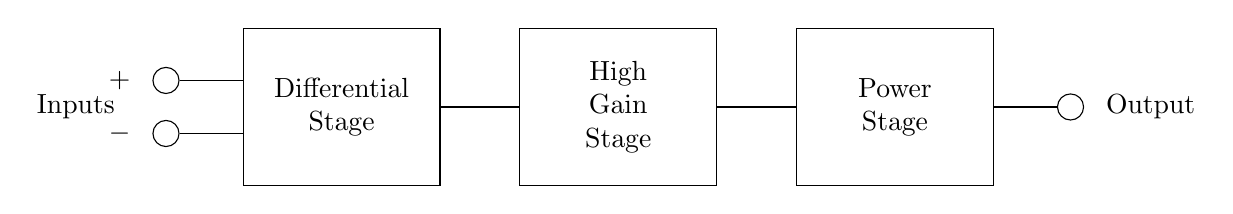
\begin{tikzpicture}
	\draw[every node/.style={draw,minimum height=20mm,align=center,minimum width=25mm}]
	node (one) {Differential\\Stage}
	node[right=of one] (two)  {High\\Gain\\Stage}
	node[right=of two] (three)  {Power\\Stage}
	(one) to (two)
	(two) to (three);
	
	\draw
	(three.east) to ++(8mm,0) node[draw,circle,anchor=west] {}
node[right=5mm] {Output};

	\draw (one.165) to ++(-8mm,0) node[draw,circle,anchor=east] {}
node[left=5mm] {+};

	\draw (one.195) to ++(-8mm,0) node[draw,circle,anchor=east] {}
node[left=5mm] {$-$};

	\node[left=15mm of one.west] {Inputs};

\end{tikzpicture}
\end{document}